% !TEX TS-program = pdflatexmk

\pdfminorversion=6

\documentclass[14pt,aspectratio=169]{beamer}
\usepackage{newtxtext,newtxmath}
\usepackage{microtype}
\usepackage[english]{babel}
\usepackage{array}
\usepackage{booktabs}
\usepackage{graphicx}
\usepackage{graphbox}
\usepackage{tikz}
\usetikzlibrary{fit}
\usetikzlibrary{positioning}
\usetikzlibrary{shapes}
\usetikzlibrary{shapes.multipart}
\usetikzlibrary{calc}
\usetikzlibrary{tikzmark}
\usetikzlibrary{backgrounds}
\usetikzlibrary{overlay-beamer-styles}
\usepackage{pgfplots}
\usepackage{forest}
\usepackage[linesnumbered,noend]{algorithm2e}
\usepackage[style=authoryear,maxbibnames=99,sorting=nyt,uniquename=false,backend=biber]{biblatex}
\AtEveryBibitem{\clearfield{note}}


%\includeonlyframes{current}

\addbibresource{bethard.bib}
\addbibresource{extra.bib}
\renewcommand*{\bibfont}{\scriptsize}
\newcommand{\subtitlecite}[1]{{\hskip0pt plus 1filll \scriptsize\parencite{#1}}}
\newcommand{\headshot}[3]{{\tiny\setlength{\tabcolsep}{0pt}%
\begin{tabular}{c}
\includegraphics[height=.2\textheight]{#1} \\
#2 \\
#3
\end{tabular}}}
\newcommand{\sectionbox}{%
\centering
\begin{beamercolorbox}[sep=8pt,center,shadow=true,rounded=true]{title}
  \usebeamerfont{title}\insertsectionhead\par%
\end{beamercolorbox}
\vspace{.2\textheight}}

% Define UA colors
% https://brand.arizona.edu/applying-the-brand/colors
\definecolor{ua-red}{HTML}{AB0520}
\definecolor{ua-blue}{HTML}{0C234B}
\definecolor{ua-oasis}{HTML}{378DBD}
\definecolor{geonames-blue}{HTML}{5c9bcc}
\colorlet{event}{ua-red}
\colorlet{time}{ua-blue}
\colorlet{partialtime}{time!50!white}

\tikzset{
  hid/.style 2 args={
    rectangle split,
    rectangle split horizontal,
    draw=#2,
    rectangle split parts=#1,
    fill=#2!40,
    outer sep=1pt},
}
\pgfplotsset{compat=1.18}

\mode<presentation>{
\usetheme{Madrid}
\usecolortheme[named=ua-red]{structure}
\setbeamertemplate{navigation symbols}{}
\setbeamertemplate{footline}[frame number]
\setbeamertemplate{section in toc}[square]
\setbeamertemplate{subsection in toc}[square]
\setbeamertemplate{items}[square]
}

% smaller than \strut, but ensures a constant height
\newcommand{\fullheight}{\vphantom{(p}}

\newcommand{\raisegraphics}[3]{\raisebox{-#1\height}{\includegraphics[#2]{#3}}}
\newcommand{\funding}[2]{\raisegraphics{.2}{height=.05\textheight}{#1} #2}


% command for annotating words in text
% #1: drawing options
% #2: name of entire shape
% #3: number of parts
% #4: name of baseline part
% #5: annotation type
% #6: node text following \nodepart{two}
\newcommand{\annotate}[6][]{%
\tikz[remember picture,baseline={(#2.#4)}]{%
\node[
  rectangle split,
  rectangle split parts=#3,
  thick,
  inner sep=2pt,
  align=center,
  draw=event,
  #1]%
(#2)
{%
\scriptsize\fullheight\textsc{#5}%
\nodepart{two}%
#6%
\fullheight};}}

% short commands for annotations of various sizes
\newcommand{\AnnotateOne}[3][]{%
  \tikz[remember picture,baseline={(#2.base)}]{%
    \node[draw,inner sep=2pt,#1] (#2) {#3\strut};%
  }%
}
\newcommand{\AnnotateTwo}[4][]{\annotate[#1]{#2}{2}{two}{#3}{#4}}
\newcommand{\AnnotateThree}[5][]{\annotate[#1]{#2}{3}{three}{#3}{%
\scriptsize\fullheight\textsc{#4}%
\nodepart{three}%
#5}}
\newcommand{\AnnotateFour}[6][]{\annotate[#1]{#2}{4}{four}{#3}{%
\scriptsize\fullheight\textsc{#4}%
\nodepart{three}%
\scriptsize\fullheight\textsc{#5}%
\nodepart{four}%
#6}}
\newcommand{\AnnotateFive}[7][]{\annotate[#1]{#2}{5}{five}{#3}{%
\scriptsize\fullheight\textsc{#4}%
\nodepart{three}%
\scriptsize\fullheight\textsc{#5}%
\nodepart{four}%
\scriptsize\fullheight\textsc{#6}%
\nodepart{five}%
#7}}
\newcommand{\AnnotateSix}[8][]{\annotate[#1]{#2}{6}{six}{#3}{%
\scriptsize\fullheight\textsc{#4}%
\nodepart{three}%
\scriptsize\fullheight\textsc{#5}%
\nodepart{four}%
\scriptsize\fullheight\textsc{#6}%
\nodepart{five}%
\scriptsize\fullheight\textsc{#7}%
\nodepart{six}%
#8}}


% command for adding links
% #1: drawing options (typically, the color)
% #2: edge options (typically out=NN, in=NN)
% #3: start anchor for arrow
% #4: end anchor for arrow
\newcommand{\AnnotateLink}[4][]{%
\path[color=time,thick,->,#1] (#3) node [circle,color=time,fill,inner sep=0.25ex,#1] {} edge[#2] (#4);}


% command for drawing a timeline
% #1: drawing options
% #2: number of primary intervals
% #3: number of secondary intervals per primary interval
\newcommand{\tikztimeline}[3][]{%
\pgfmathsetmacro{\primaryend}{#2-1}
\pgfmathsetmacro{\secondaryend}{#3-1}
% horizontal line
\draw[#1,dashed] (-0.33,0) -- (0,0);
\draw[#1] (0,0) -- (#2,0);
\draw[#1,dashed,-latex] (#2,0) -- (#2 + 0.33,0);
% primary ticks
\foreach \primary  in {0,...,\primaryend} {%
  \draw[#1] (\primary,0) -- (\primary,\normalbaselineskip);
  % secondary ticks
  \foreach \secondary [evaluate=\secondary] in {\primary+1/#3,\primary+.../#3,\primary+\secondaryend/#3} {
    \draw[#1] (\secondary,0) -- (\secondary,0.5\normalbaselineskip);
  }
}
\draw[#1] (#2,0) -- (#2,\normalbaselineskip);
}

% command for drawing a interval on a timeline
% #1: drawing options
% #2: start time (i.e., start x position)
% #3: end time (i.e., start x position)
% #4: vertical tier (i.e., y position)
% #5: text
\newcommand{\tikztimelineinterval}[5][]{%
\draw[line width=0.9\normalbaselineskip,draw=time,text=white,#1] (#2, #4\normalbaselineskip) -- (#3, #4\normalbaselineskip) node[midway,font=\footnotesize] {#5};
}

% short command for drawing an interval the width of a single primary interval
\newcommand{\tikztimelineprimaryinterval}[4][]{\tikztimelineinterval[#1]{#2}{#2+1}{#3}{#4}}

\newcommand{\xml}[2]{\texttt{{\textless}#1{\textgreater}}#2\texttt{{\textless}/#1{\textgreater}}}

\author[Bethard]{Steven Bethard, Ph.D.}
\institute[Arizona]{Associate Professor \\ College of Information Science \\ University of Arizona}

\title{Can large language models understand language-external structures?}
\date[]{25 Jun 2025}

\begin{document}


\begin{frame}
  \titlepage
\end{frame}

\begin{frame}[t]{Large language models vs. timelines}
\centering
\begin{tikzpicture}[inner sep=0pt]
\node (chatgpt) {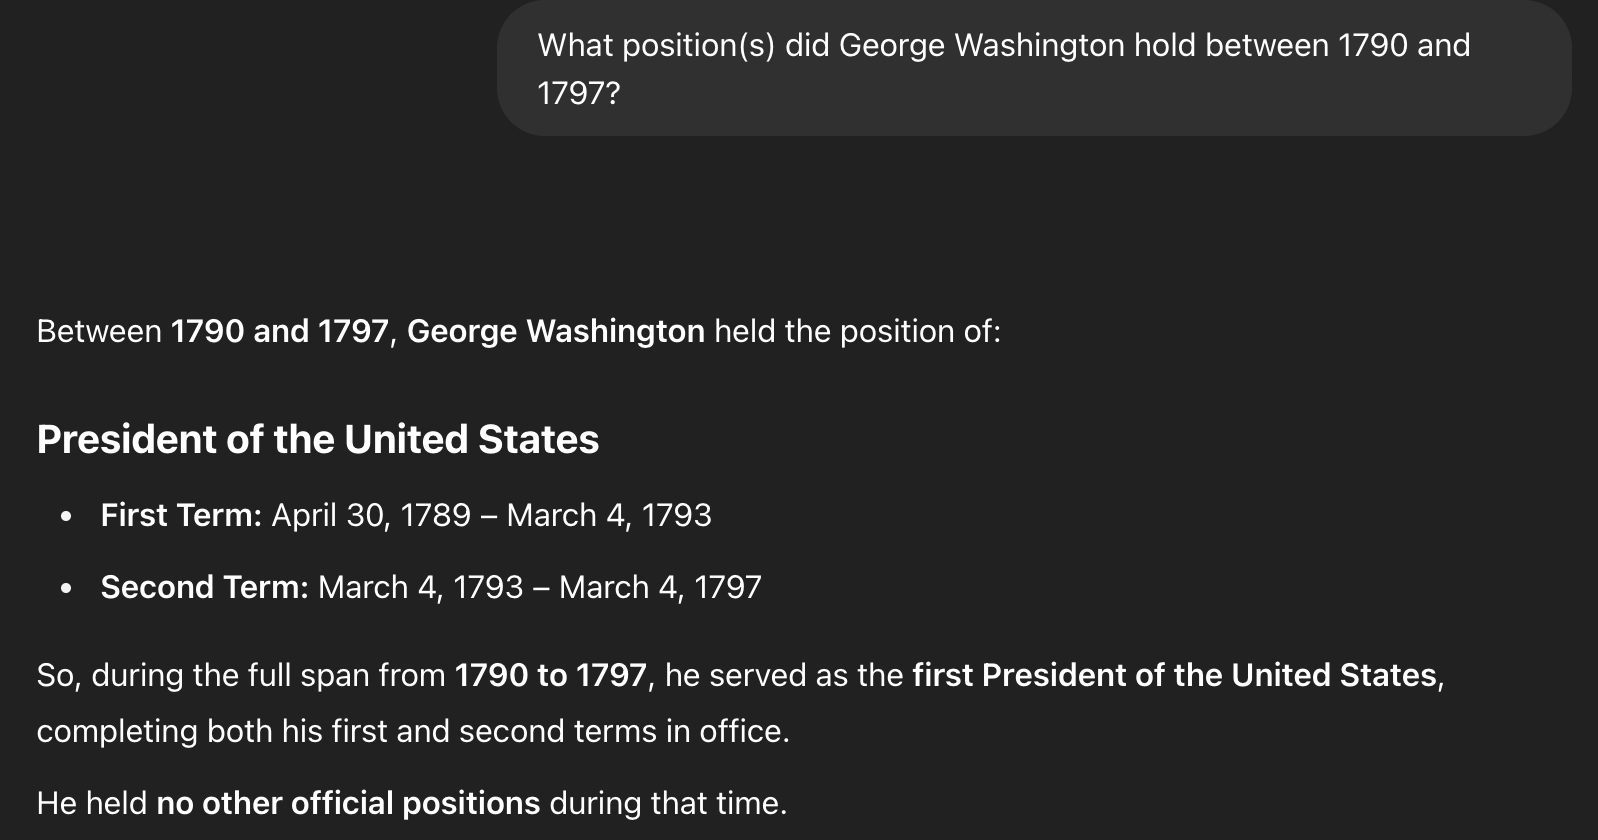
\includegraphics[width=.8\textwidth]{chatgpt/timeline.png}};
\pause
\node[draw] (calendar1) at (chatgpt) {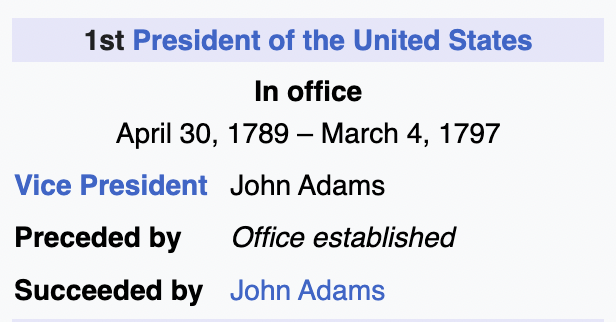
\includegraphics[width=.45\textwidth]{timeline/washington-president.png}};
\node[draw, anchor=north] (calendar2) at (calendar1.south) {
\includegraphics[width=.45\textwidth]{timeline/washington-chancellor.png}};
\end{tikzpicture}
\end{frame}

\begin{frame}[t]{Large language models vs. maps}
\centering
\begin{tikzpicture}[inner sep=0pt]
\node (chatgpt) {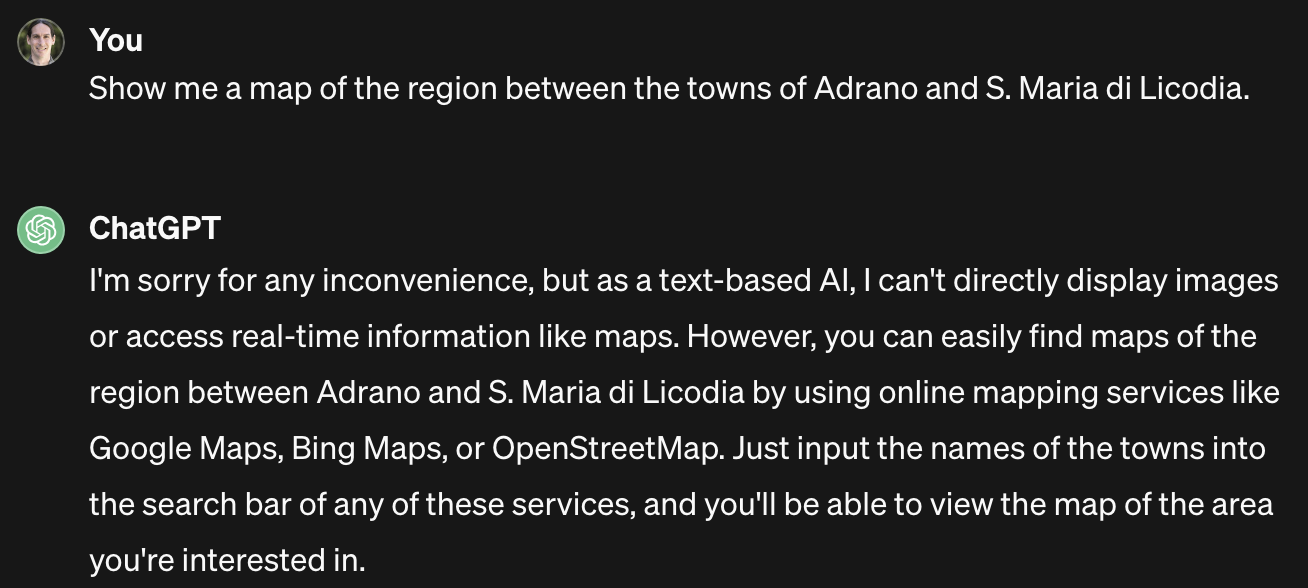
\includegraphics[width=.8\textwidth]{chatgpt/map.png}};
\pause
\node[draw, yshift=1cm] (map) at (chatgpt.south) {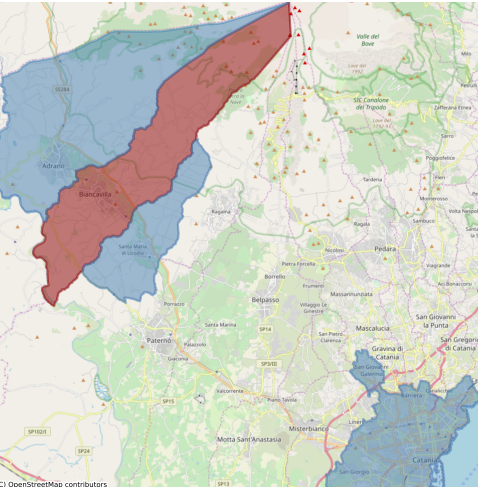
\includegraphics[width=.3\textwidth]{compgeo/map-biancavilla-out.png}};
\end{tikzpicture}
\end{frame}

\begin{frame}[t]{Large language models vs. ontologies}
\centering
\begin{tikzpicture}[inner sep=0pt]
\node (chatgpt) {
\includegraphics[width=.8\textwidth]{chatgpt/snomed.png}};
\pause
\node[draw, xshift=1cm] (snomed1) at (chatgpt.south) {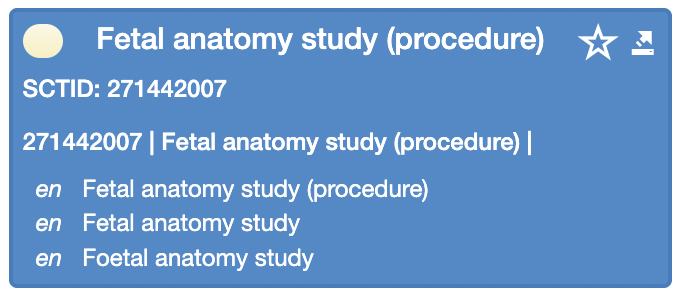
\includegraphics[width=.4\textwidth]{snomed/fetal-anatomy-study.png}};
\pause
\node[draw, anchor=north] (snomed2) at (snomed1.north) {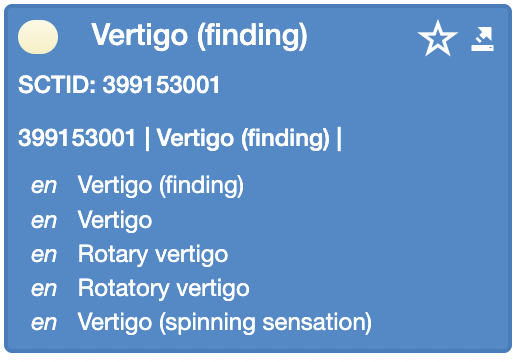
\includegraphics[width=.4\textwidth]{snomed/vertigo.png}};
\end{tikzpicture}
\end{frame}

%\begin{frame}{My natural language processing research interests}
%\begin{itemize}
%\item Modeling the language of time and timelines \\
%{\footnotesize Funded by:
%\funding{funding/nih_nlm.png}{R01LM010090}
%\quad\funding{funding/darpa.png}{W911NF-18-1-0014}}
%\begin{itemize}
%% image generated from https://demo.mobiscroll.com/jquery/calendar/multiple-select
%\item E.g., \textit{six days ago} $\Rightarrow$ \raisegraphics{.4}{height=.15\textheight}{calendar/2024-02-07.png}
%\end{itemize}
%
%\bigskip
%\item Normalizing text to medical and geospatial ontologies \\
%{\footnotesize Funded by:
%\funding{funding/nih_nigms.jpg}{R01GM114355}
%\quad\funding{funding/nsf.png}{1831551}}
%\begin{itemize}
%\item E.g., \textit{Boulder} $\Rightarrow$ \raisegraphics{.4}{height=.15\textheight}{geonames/BoulderUSCOP.png}
%\end{itemize}
%
%\bigskip
%\item Adapting machine learning models to medical and clinical domains \\
%{\footnotesize Funded by:
%\funding{funding/nih_nlm.png}{R01LM012918}
%\quad\funding{funding/nih_nci.jpg}{R21CA256680}}
%\end{itemize}
%\end{frame}


\begin{frame}
    \frametitle{Talk Outline: Lessons and Opportunities}
    \tableofcontents
\end{frame}

\section{Lesson 1: Structured~Pre-training \textgreater\ Unstructured~Pre-training}

\begin{frame}[b]
\sectionbox
\funding{funding/nih_nigms.jpg}{R01GM114355}
\hfill
\headshot{people/xu-dongfang.jpeg}{Dongfang Xu, Ph.D.}{Doctoral student}
\end{frame}

\subsection{Medical concept normalization}

\begin{frame}[t]{Concept normalization: text term $\Rightarrow$ ontology entry}
\centering
I felt like \AnnotateTwo[draw=ua-red]{vomiting}{\visible<2->{C0042963}}{vomiting}, and my \AnnotateTwo[draw=ua-red]{spinning}{\visible<2->{C0012833}}{head was spinning a little}.

\bigskip
\only<3->{
\begin{tikzpicture}[remember picture,overlay]
\node[anchor=north, inner sep=0pt, below=2em of vomiting.south]
  (umls-vomiting)
  {
\includegraphics[width=0.35\textwidth]{umls/vomiting.png}}
  edge[ua-red,ultra thick,dotted,latex-] (vomiting);
\node[anchor=north, inner sep=0pt, below=2em of spinning.south]
  (umls-dizziness)
  {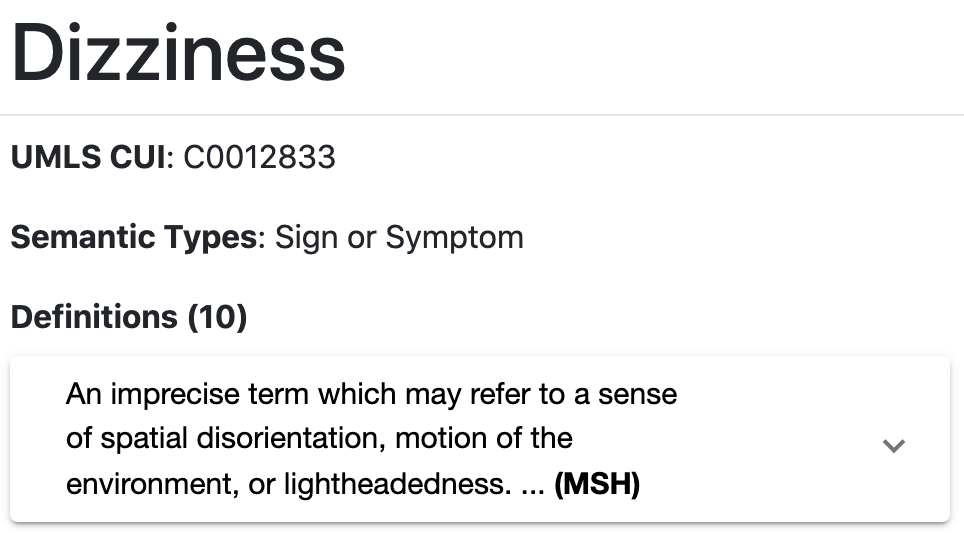
\includegraphics[width=0.35\textwidth]{umls/dizziness.png}}
  edge[ua-red,ultra thick,dotted,latex-] (spinning);
\node[draw,fit=(umls-vomiting) (umls-dizziness), inner sep=1em, label=below:{Unified Medical Language System (UMLS)}] {};
\end{tikzpicture}
}
\end{frame}

\begin{frame}{Concept normalization \textless\ 2021: retrieve + rerank}
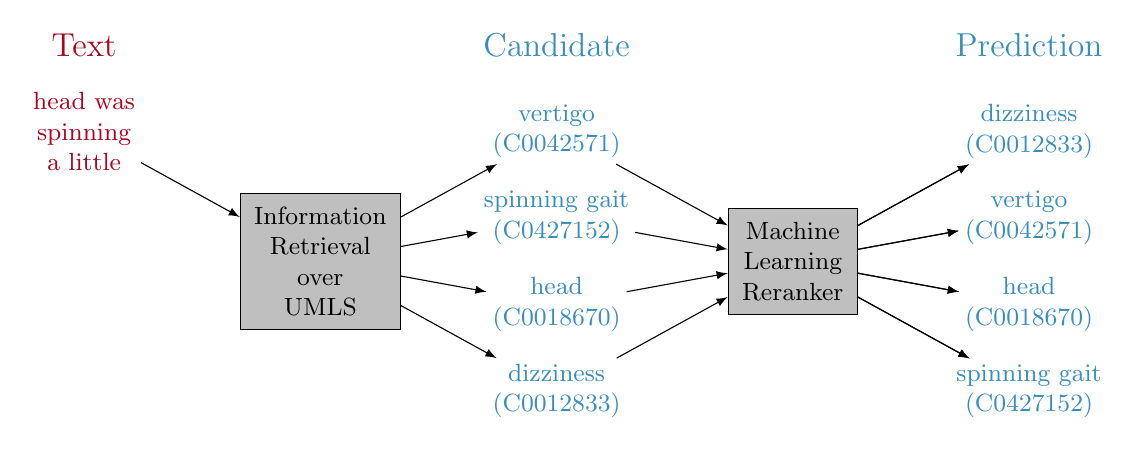
\begin{tikzpicture}[font=\small, inner sep=2pt, model/.style={draw, fill=black!25, align=center, inner sep=5pt}]
\pgfmathsetseed{42}
\pgfmathsetmacro{\height}{1.1}
\pgfmathsetmacro{\width}{3}

\node[ua-red] at (0, \height) {\large Text};
\node[ua-oasis] at (2*\width, \height) {\large Candidate};
\node<2->[ua-oasis] at (4*\width, \height) {\large Prediction};

\node[ua-red, align=center] (text) at (0, 0) {head was \\ spinning \\ a little};
\node[model] (umls) at (\width, -1.5*\height) {Information \\ Retrieval \\ over \\ UMLS} edge[latex-] (text);
\node<2->[model] (reranker) at (3*\width, -1.5*\height) {Machine \\ Learning \\ Reranker};
\foreach[count=\i from 0, count=\slide from 4] \candidate/\prediction in {
    vertigo\\(C0042571)/dizziness\\(C0012833),
    spinning gait\\(C0427152)/vertigo\\(C0042571),
    head\\(C0018670)/head\\(C0018670),
    dizziness\\(C0012833)/spinning gait\\(C0427152)} {
  \node[ua-oasis, align=center] (candidate-\i) at (2*\width, -\height*\i) {\candidate};
  \draw[-latex] (umls) -- (candidate-\i);
  \draw<2->[-latex] (candidate-\i) -- (reranker);
  \node<2->[ua-oasis, align=center] (prediction-\i) at (4*\width, -\height*\i) {\prediction} edge[latex-] (reranker);
  \draw<2->[-latex] (reranker) -- (prediction-\i);
}
\end{tikzpicture}
\end{frame}


\begin{frame}{Concept normalization as vector-space search}
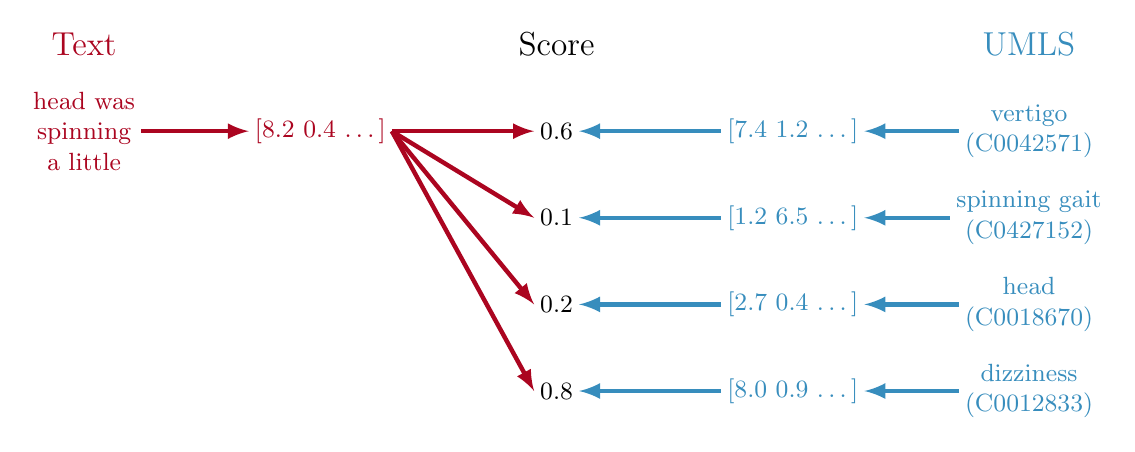
\begin{tikzpicture}[font=\small, inner sep=2pt]
\pgfmathsetseed{42}
\pgfmathsetmacro{\height}{1.1}
\pgfmathsetmacro{\width}{3}

\node[ua-red] at (0, \height) {\large Text};
\node<4-> at (2*\width, \height) {\large Score};
\node[ua-oasis] at (4*\width, \height) {\large UMLS};

\node[align=center,ua-red] (text) at (0, 0) {head was \\ spinning \\ a little};
\node<2->[ua-red] (text-vec) at (\width, 0) {\small[8.2 0.4 \ldots]}
  edge[ua-red, ultra thick, latex-] (text);
\foreach[count=\i from 0, count=\slide from 4] \term/\vec/\score in {
    vertigo\\(C0042571)/[7.4 1.2 \ldots]/0.6,
    spinning gait\\(C0427152)/[1.2 6.5 \ldots]/0.1,
    head\\(C0018670)/[2.7 0.4 \ldots]/0.2,
    dizziness\\(C0012833)/[8.0 0.9 \ldots]/0.8} {
  \node[ua-oasis, align=center] (umls-\i) at (4*\width, -\height*\i) {\term};
  \node<3->[ua-oasis] (umls-vec-\i) at (3*\width, -\height*\i) {\vec}
    edge[ua-oasis, ultra thick, latex-] (umls-\i);
  \node<\slide-> (score-\i) at (2*\width, -\height*\i) {\score}
    edge[ua-oasis, ultra thick, latex-] (umls-vec-\i);
  \draw<\slide->[ua-red, ultra thick, -latex] (text-vec.east) -- (score-\i.west);
}
\end{tikzpicture}
\end{frame}

\begin{frame}{Training term-to-vector language models on UMLS}{\subtitlecite{xu-bethard-2021-triplet}}
\begin{enumerate}
\item Create triplets of input term $t_i$, match term $t_p$, mis-match term $t_n$
\item Train network so $t_i$ is more similar to $t_p$ than $t_n$
\end{enumerate}

\pause
\bigskip
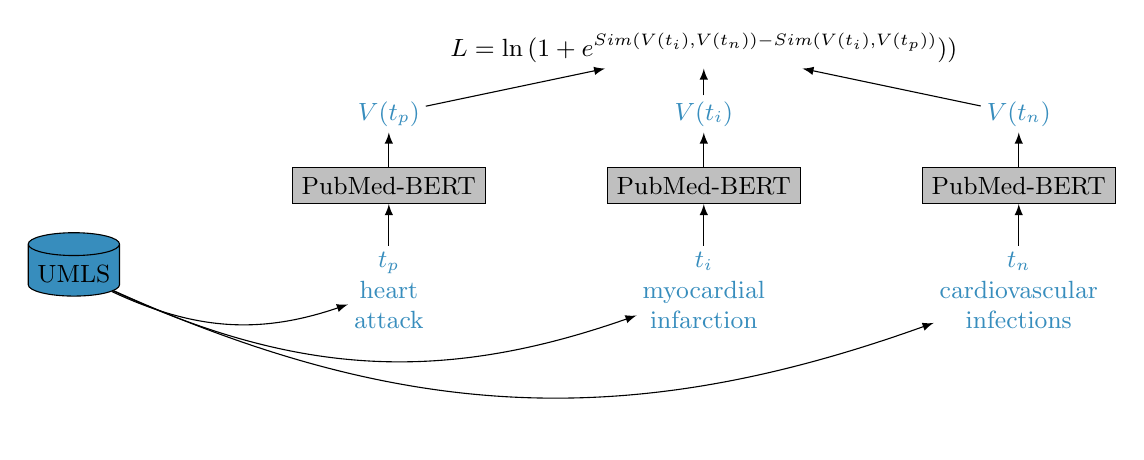
\begin{tikzpicture}[font=\small, text only/.style={inner sep=2pt, align=center}]
\pgfmathsetmacro{\height}{1.4}
\pgfmathsetmacro{\width}{1}
\node[draw, fill=ua-oasis, cylinder, shape border rotate=90, shape aspect=.25, align=center]
  (umls)
  at (-8*\width, .15*\height)
  {UMLS};
\node[text only]
  (L)
  at (0, 2.2*\height)
  {$L = \ln{(1 + e^{Sim(V(t_i), V(t_{n})) - Sim(V(t_i), V(t_{p}))} )})$};
\foreach \i/\name/\textcolor/\phrase in {
    -4/p/ua-oasis/heart\\attack,
    0/i/ua-oasis/myocardial\\infarction,
    4/n/ua-oasis/cardiovascular\\infections} {
  \node[text only, text=\textcolor]
    (input-\name)
    at (\i*\width, 0)
    {$t_{\name}$ \\ \phrase} edge[latex-,bend left=22] (umls);
  \node[draw, align=center, fill=black!25]
    (bert-\name)
    at (\i*\width, 0.95*\height)
    {PubMed-BERT}
    edge[latex-] (input-\name);
  \node[text only,text=\textcolor]
    (repr-\name)
    at (\i*\width, 1.6*\height)
    {$V(t_{\name})$}
    edge[latex-] (bert-\name)
    edge[-latex] (L);
}
\end{tikzpicture}
\end{frame}

\begin{frame}{Concept normalization evaluation data}
\begin{description}[NCBI]
\item[NCBI] disorders, MEDIC, PubMed abstracts
\item[B-D] diseases, MEDIC, BioCreative V challenge
\item[B-C] chemicals, CTD, BioCreative V challenge
\item[S/C] disorders, UMLS, ShARe/CLEF eHealth 2013
\item[MCN] various concepts, UMLS, 2019 n2c2 Shared-Task
\end{description}
\end{frame}

\begin{frame}{Structured pre-training \textgreater\ unstructured pre-training}{\subtitlecite{xu-bethard-2021-triplet}}
\begin{tabular}{ l c c c c c c}
\toprule
Approach & NCBI & B-D & B-C  & S/C & MCN \\
\midrule
PubMedBERT & \alert<2>{76.6}  & \alert<2>{76.7} & \alert<2>{91.8}  & \alert<2>{73.6}  & \alert<2>{60.0} \\
PubMedBERT + Train:O & \alert<2-3>{82.6}  & \alert<2-3>{84.4} & \alert<2-3>{95.8} & \alert<2-3>{83.5} &  \alert<2-3>{69.6}  \\
PubMedBERT + Train:O + Search:T & \alert<3>{89.5} & \alert<3>{92.3} & \alert<3>{96.7} & \alert<3>{89.2} &  \alert<3>{82.2}  \\
\bottomrule
\end{tabular}

\quad O = Ontology; T = target domain terms

\bigskip
Findings:
\begin{itemize}
\item<2-> Triplet-training on ontology yields better language model
\item<3-> Adding new terms to the ontology helps even without retraining
\end{itemize}
\end{frame}


\section{Lesson 2: Structured~Prompt \textgreater\ Structured~Network}

\begin{frame}[b]
\sectionbox
\funding{funding/nih_nlm.png}{R01LM010090}
\hfill
\headshot{people/su-xin.jpg}{Xin Su}{Doctoral student}
\end{frame}

\subsection{Timeline-based question answering}

\begin{frame}{Timeline-based question answering with LLMs}
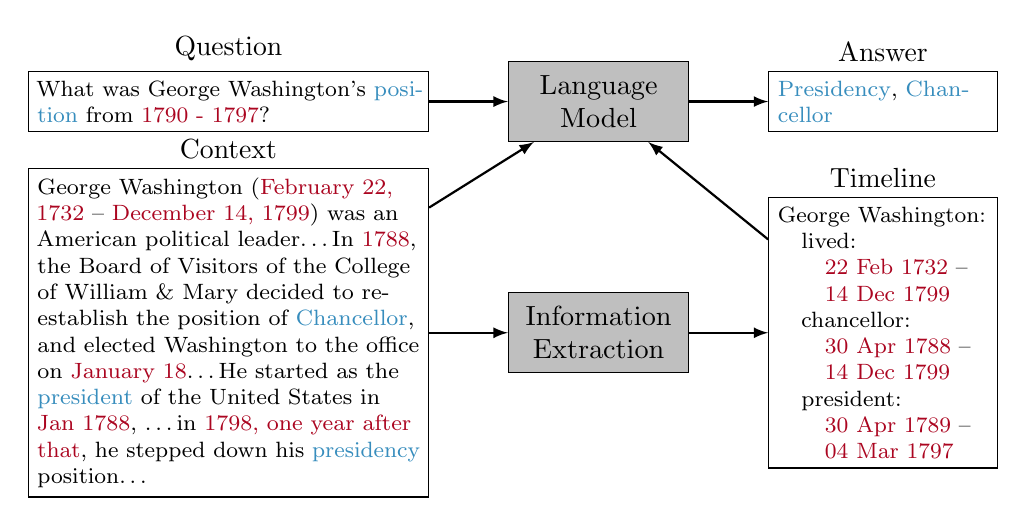
\begin{tikzpicture}[
  note/.style={draw, font=\footnotesize},
  model/.style={draw, fill=black!25, align=center, inner sep=5pt, text width=.16\textwidth}
]

\node[note, text width=.4\textwidth, label=Question] (question) at (0, 0) {%
What was George Washington’s \textcolor{ua-oasis}{position} from \textcolor{ua-red}{1790 - 1797}?};

\node[note, text width=.4\textwidth, below=3ex of question, label=Context] (context) {%
George Washington (\textcolor{ua-red}{February 22, 1732} -- \textcolor{ua-red}{December 14, 1799}) was an American political leader\ldots
%Congress created the Continental Army on June 14, 1775, and Samuel and John Adams nominated Washington to become its Commander-in-Chief\ldots
%Washington bade farewell to his officers at Fraunces Tavern in December 1783 and resigned his commission days later.
In \textcolor{ua-red}{1788}, the Board of Visitors of the College of William \& Mary decided to re-establish the position of \textcolor{ua-oasis}{Chancellor}, and elected Washington to the office on \textcolor{ua-red}{January 18}\ldots
He started as the \textcolor{ua-oasis}{president} of the United States in \textcolor{ua-red}{Jan 1788}, \ldots in \textcolor{ua-red}{1798, one year after that}, he stepped down his \textcolor{ua-oasis}{presidency} position\ldots};

\node[model, right=of question] (model)  {Language \\ Model};

\visible<2->{\node[model, right=of context] (ie)  {Information \\ Extraction};}

\visible<2->{\node[note, text width=.22\textwidth, label=Timeline, right=of ie] (timeline)  {%
George Washington:\\
\quad lived: \\
\qquad \textcolor{ua-red}{22 Feb 1732} --\\
\qquad \textcolor{ua-red}{14 Dec 1799}\\
\quad chancellor: \\
\qquad \textcolor{ua-red}{30 Apr 1788} -- \\
\qquad \textcolor{ua-red}{14 Dec 1799}\\
\quad president: \\
\qquad \textcolor{ua-red}{30 Apr 1789} -- \\
\qquad \textcolor{ua-red}{04 Mar 1797}};}

\node[note, text width=.22\textwidth, label=Answer, right=of model] (answer) {%
\textcolor{ua-oasis}{Presidency}, \textcolor{ua-oasis}{Chancellor}};

\visible<2->{\draw[thick, -latex] (context) -- (ie);}
\visible<2->{\draw[thick, -latex] (ie) -- (timeline);}
\draw[thick, -latex] (question) -- (model);
\draw[thick, -latex] (context) -- (model);
\visible<2->{\draw[thick, -latex] (timeline) -- (model);}
\draw[thick, -latex] (model) -- (answer);
\end{tikzpicture}
\end{frame}

\begin{frame}{Injecting timelines into LLMs via graph networks}
\begin{tikzpicture}[
  note/.style={draw, align=left, font=\scriptsize},
  event/.style={note, inner sep=2pt, ua-oasis},
  time/.style={note, inner sep=2pt, ua-red},
  model/.style={draw, fill=black!25, align=center, inner sep=5pt, text width=.2\textwidth}
]

% Question
\node[note, anchor=north, text width=.49\textwidth, label=Input] (question) at (0, 0) {%
What was George Washington’s \textcolor{ua-oasis}{position} from \textcolor{ua-red}{1790 - 1797}?};

% Context
\node[note, text width=.49\textwidth, below=.8ex of question] (context) {%
George Washington (\textcolor{ua-red}{February 22, 1732} -- \textcolor{ua-red}{December 14, 1799}) was an American political leader\ldots
In \textcolor{ua-red}{1788}, the Board of Visitors of the College of William \& Mary decided to re-establish the position of \textcolor{ua-oasis}{Chancellor}, and elected Washington to the office on \textcolor{ua-red}{January 18}\ldots
He started as the \textcolor{ua-oasis}{president} of the\ldots
%United States in \textcolor{ua-red}{Jan 1788}, \ldots in \textcolor{ua-red}{1798, one year after that}, he stepped down his \textcolor{ua-oasis}{presidency} position\ldots
};

% Timeline
\node[note, text width=.49\textwidth, text height=.35\textheight, below=.8ex of context] (timeline) {};
\node[time] (qt) at (-2.8, -4) {1790 -- 1797};
\node[event, below=of qt] (qe) {position\\(What)};
\node[time, right=1.5ex of qt] (dt2) {1788};
\node[event, below=of dt2] (de2) {re-establish\\(Chancellor)};
\node[time, right=3ex of dt2] (dt3) {18 Jan 1788};
\node[event, below=of dt3] (de3) {elected\\(Chancellor)};
\node[time, right=1.5ex of dt3] (dt4) {Jan 1788};
\node[event, below=of dt4] (de4) {started\\(president)};
\node[right=.5ex of dt4] (timelinedots) {\ldots};
%\node[time, right=1ex of dt4] (dt5) {1798};
%\node[event, below=of dt5] (de5) {stepped down\\(president)};
\draw (qt) edge[thick, -latex] node[above, sloped, font=\tiny]{\texttt{includes}} (qe);
\draw (dt2) edge[thick, -latex] node[above, sloped, font=\tiny]{\texttt{includes}} (de2);
\draw (dt3) edge[thick, -latex] node[above, sloped, font=\tiny]{\texttt{includes}} (de3);
\draw (dt4) edge[thick, -latex] node[above, sloped, font=\tiny]{\texttt{includes}} (de4);
\draw (dt3.north) edge[thick, -latex, out=150, in=30] node[very near start, above, sloped, font=\tiny]{\texttt{before}} (qt.north);
\draw (dt4.north) edge[thick, -latex, out=150, in=30] node[very near start, above, sloped, font=\tiny]{\texttt{before}} (qt.north);

% Network
\node[hid={8}{black}, right=of question, label=Language Model] (layer0) {};
\node[model, below=1.4ex of layer0] (gnn) {RelGraphConv};
\node[hid={8}{black}, below=1.4ex of gnn] (layer1) {};
\node[model, below=1.4ex of layer1] (transformer0) {Transformer};
\node[below=1.4ex of transformer0] (dots) {...};
\node[model, below=1.4ex of dots] (transformer1) {Transformer};
\node[hid={8}{black}, below=1.4ex of transformer1] (layer2) {};
\draw[thick, -latex] (layer0) to (gnn);
\draw[thick, -latex] (gnn) to (layer1);
\draw[thick, -latex] (layer1) to (transformer0);
\draw[thick, -latex] (transformer1) to (layer2);

% Edges
\draw[thick, -latex] (question.east) to (layer0.west);
\draw[thick, -latex] (context.east) to (layer0.west);
\draw[thick, -latex] (timeline.east) to (gnn.west);
\end{tikzpicture}
\end{frame}


\begin{frame}{Injecting timelines into LLMs via structured prompts}
\begin{tikzpicture}[
  note/.style={draw, align=left, font=\scriptsize},
  event/.style={note, inner sep=2pt, ua-oasis},
  time/.style={note, inner sep=2pt, ua-red},
  model/.style={draw, fill=black!25, align=center, inner sep=5pt, text width=.25\textwidth}
]

% Question
\node[note, anchor=north, text width=.49\textwidth, label=Input] (question) at (0, 0) {%
What was George Washington’s \textcolor{ua-oasis}{position} from \textcolor{ua-red}{1790 - 1797}?};

% Context
\node[note, text width=.49\textwidth, below=.8ex of question] (context) {%
George Washington (\textcolor{ua-red}{February 22, 1732} -- \textcolor{ua-red}{December 14, 1799}) was an American political leader\ldots
In \textcolor{ua-red}{1788}, the Board of Visitors of the College of William \& Mary decided to re-establish the position of \textcolor{ua-oasis}{Chancellor}, and elected Washington to the office on \textcolor{ua-red}{January 18}\ldots
He started as the \textcolor{ua-oasis}{president} of the\ldots
%United States in \textcolor{ua-red}{Jan 1788}, \ldots in \textcolor{ua-red}{1798, one year after that}, he stepped down his \textcolor{ua-oasis}{presidency} position\ldots
};

% Timeline
\node[note, text width=.49\textwidth, text height=.35\textheight, below=.8ex of context] (timeline) {};
\node[time] (qt) at (-2.8, -4) {1790 -- 1797};
\node[event, below=of qt] (qe) {position\\(What)};
\node[time, right=1.5ex of qt] (dt2) {1788};
\node[event, below=of dt2] (de2) {re-establish\\(Chancellor)};
\node[time, right=3ex of dt2] (dt3) {18 Jan 1788};
\node[event, below=of dt3] (de3) {elected\\(Chancellor)};
\node[time, right=1.5ex of dt3] (dt4) {Jan 1788};
\node[event, below=of dt4] (de4) {started\\(president)};
\node[right=.5ex of dt4] (timelinedots) {\ldots};
%\node[time, right=1ex of dt4] (dt5) {1798};
%\node[event, below=of dt5] (de5) {stepped down\\(president)};
\draw (qt) edge[thick, -latex] node[above, sloped, font=\tiny]{\texttt{includes}} (qe);
\draw (dt2) edge[thick, -latex] node[above, sloped, font=\tiny]{\texttt{includes}} (de2);
\draw (dt3) edge[thick, -latex] node[above, sloped, font=\tiny]{\texttt{includes}} (de3);
\draw (dt4) edge[thick, -latex] node[above, sloped, font=\tiny]{\texttt{includes}} (de4);
\draw (dt3.north) edge[thick, -latex, out=150, in=30] node[very near start, above, sloped, font=\tiny]{\texttt{before}} (qt.north);
\draw (dt4.north) edge[thick, -latex, out=150, in=30] node[very near start, above, sloped, font=\tiny]{\texttt{before}} (qt.north);

% Prompt
\node[note, anchor=north, text width=.41\textwidth, label=Prompt] (prompt) at (7.9, 0) {%
\texttt{question}:
What was George Washington’s position from \textcolor{ua-red}{\xml{question\_time}{1790 - 1797}}? \\
\texttt{context}: \ldots
George Washington (\textcolor{ua-red}{\xml{before}{February 22, 1732}} -- \textcolor{ua-red}{\xml{after}{December 14, 1799}}) was an American political leader\ldots
In \textcolor{ua-red}{\xml{before}{1788}}, the Board of Visitors of the College of William \& Mary decided to re-establish the position of Chancellor, and elected Washington to the office on \textcolor{ua-red}{\xml{before}{January 18}}\ldots
He started as the president of the United States in \textcolor{ua-red}{\xml{before}{Jan 1788}}, \ldots
In \textcolor{ua-red}{\xml{after}{1798, one year after that}}, he stepped down his presidency position\ldots
};

% Language Model
\node[model, below=1.8ex of prompt] (model) {Language Model};

% Edges
\draw[thick, -latex] (question.east) to (prompt);
\draw[thick, -latex] (context.east) to (prompt);
\draw[thick, -latex] (timeline.east) to (prompt);
\draw[thick, -latex] (prompt.south) to (model);
\end{tikzpicture}
\end{frame}

\begin{frame}{Time question answering evaluation data}
\begin{description}[\ ]
\item[TimeQAEasy] {\small\parencite{chen2021a}} \\
synthetic questions over Wikipedia, times mentioned in text  \\
E.g., \textit{Which organization owned Razorfish (company) from 2007 to 2009?}
\item[TimeQAHard]  {\small\parencite{chen2021a}} \\
synthetic questions over Wikipedia, times not mentioned in text \\
E.g., \textit{Which organization owned Razorfish (company) in Feb 2007?}
\item[SituatedQA] {\small\parencite{zhang-choi-2021-situatedqa}} \\
crowdsourced questions over Wikipedia \\
E.g., \textit{Which COVID-19 vaccines have been authorized for adults in the US as of Jan 2021?}
\end{description}
\end{frame}

\begin{frame}{Structured prompt \textgreater\ structured network}
\setlength{\tabcolsep}{.3em}
\begin{tabular}{l c c c}
\toprule
& \multicolumn{3}{c}{Exact match accuracy} \\
Model
& TimeQAEasy
& TimeQAHard
& SituatedQA \\
\midrule
LongT5  & \alert<2>{55.4} & \alert<2>{49.9} & \alert<2>{24.7} \\
LongT5 + graph network  & \alert<2-3>{54.2} & \alert<2-3>{49.0} & \alert<2-3>{27.3} \\
LongT5 + structured prompt  & \alert<3>{56.9} & \alert<3>{54.0} & \alert<3>{29.0} \\
\bottomrule
\end{tabular}

\bigskip
Findings:
\begin{itemize}
\item<2-> Timelines integrated via graph networks sometimes hurt
\item<3-> Timelines integrated via structured prompts consistently help
\end{itemize}
\end{frame}



\section{Lesson 3: Predicting~Executable~Structure \textgreater\ Network~Reasoning}

\begin{frame}[b]
\sectionbox
\begin{tabular}{l}
\funding{funding/darpa.png}{W911NF-18-1-0014} \\
\funding{funding/nsf.png}{1831551}
\end{tabular}
\hfill
\headshot{people/zhang-zeyu.png}{Zeyu Zhang, Ph.D.}{Doctoral student}
\end{frame}

\subsection{Toponym resolution}

\begin{frame}{Toponym resolution: text locations $\Rightarrow$ map locations}
\centering
\textit{\AnnotateOne{sj}{San Jose} is the largest city in Northern California.}

\vspace{0.15\textheight}
\begin{tikzpicture}[remember picture]
\node (sj-cr) at (-3.5, 0) {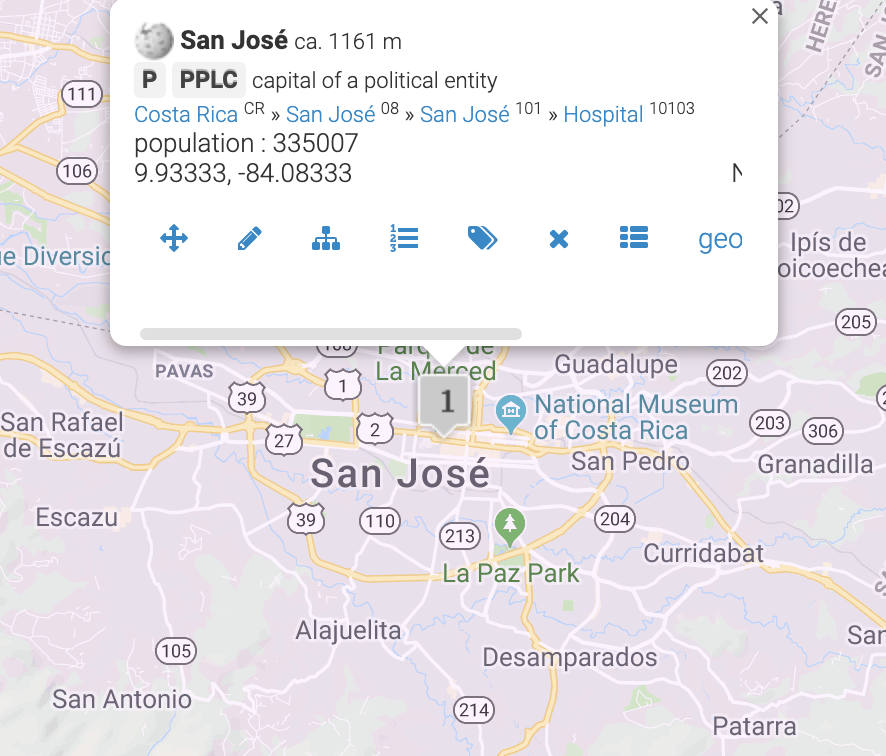
\includegraphics[width=0.65\textheight]{san-jose-costa-rica.png}};
\node (sj-us) at (+3.5, 0) {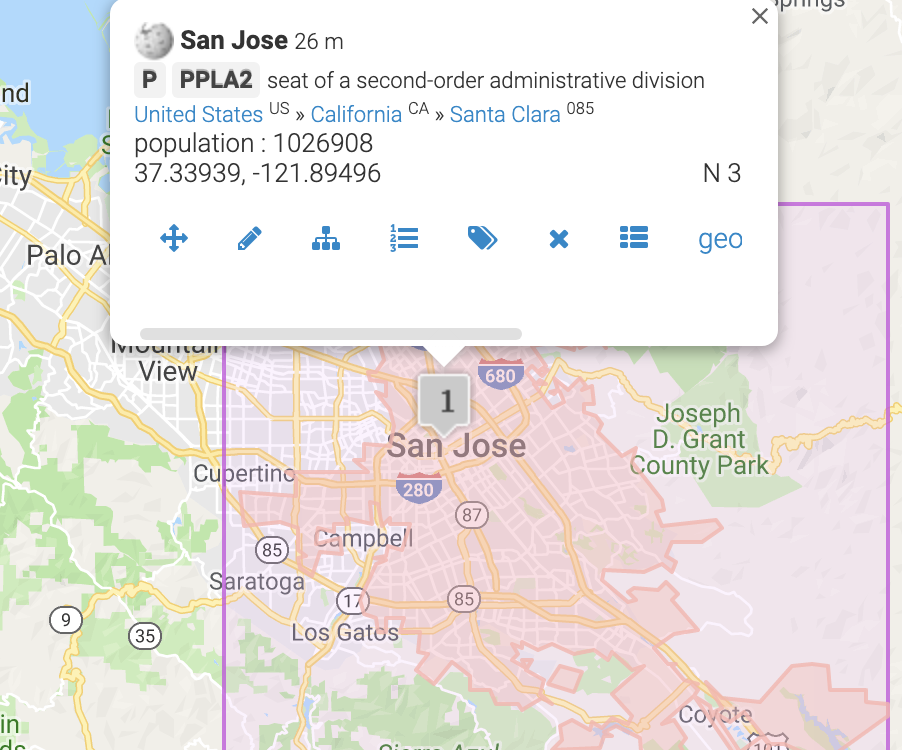
\includegraphics[width=0.65\textheight]{san-jose-california.png}};
\end{tikzpicture}
\begin{tikzpicture}[remember picture,overlay]%
\draw[-latex, ultra thick] (sj.south) -- node[red] {\Huge $\times$} (sj-cr.north);
\draw[-latex, ultra thick] (sj.south) -- (sj-us.north);
\end{tikzpicture}
\end{frame}


\begin{frame}{Toponym resolution \textless\ 2023: \\\quad retrieve entries $\Rightarrow$ classify text + entry}
\begin{tikzpicture}[
  model/.style={draw, fill=black!25, align=center, inner sep=5pt},
  geoentry/.style={inner sep=1pt, text width=0.22\linewidth, align=center},
  textforentry/.style={fill=white, inner sep=1pt, text width=0.22\linewidth, align=left},
  font=\scriptsize,
  remember picture
]
\node[draw, text width=.95\linewidth, align=left, text=ua-red] (text) at (0, 0) {It's a northeast Texas thing, not just a \subnode[inner sep=0pt]{mention}{\fbox{Paris}} thing\ldots Dallas media stations reported the same message as a hoax\ldots};

\node[model, text width=.75\linewidth] (geonames) at (0, -1) {Index (Lucene over GeoNames)}
edge[latex-] (mention.south);
\foreach \prediction/\png/\entry [count=\n from 0] in {
    % https://www.geonames.org/2988507/paris.html
    0/ParisFR11P.png/Paris [SEP] FR,
    % https://www.geonames.org/4717560/paris.html
    \fbox{1}/ParisUSTXP.png/Paris [SEP] US,
    % https://www.geonames.org/7174050/city-of-paris.html
    0/ParisUSTXA.png/City of Paris [SEP] US,
    % https://www.geonames.org/6942553/paris.html
    0/ParisCA08P.png/Paris [SEP] CA} {
    \node[draw, geoentry] (entry\n) at (-5.4 + 3.6*\n, -2.25) {\includegraphics[width=\linewidth,trim={0 0 4cm 0},clip]{geonames/\png}};
    \node[draw, textforentry, below=0.25cm of entry\n.south] (transformerin\n) {[CLS] \textcolor{geonames-blue}{\entry\ldots}\ [SEP] \textcolor{ua-red}{Paris [SEP] It's a northeast Texas\ldots}};
    \node[below=1.4cm of transformerin\n.south] (prediction\n) {\strut\prediction};
    \draw[-latex] (geonames.south) to (entry\n.north);
    \draw[-latex] (entry\n.south) to (transformerin\n.north);
    \draw[-latex] (transformerin\n.south) to (prediction\n.north);
}
\node[model, text width=.75\linewidth] (transformer) at (0, -4.4) {Classifier (Transformer Network)};
\end{tikzpicture}
\end{frame}


\begin{frame}{New Paradigm: classify text attributes $\Rightarrow$ filter entries}{\subtitlecite{zhang-etal-2024-improving-toponym}}
\begin{tikzpicture}[
  model/.style={draw, text width=.44\linewidth, fill=black!25, align=center, inner sep=5pt},
  geoentry/.style={inner sep=0pt, text width=0.35\linewidth, align=center},
  textforentry/.style={fill=white, inner sep=1pt, text width=0.45\linewidth, align=left},
  font=\scriptsize,
  remember picture
]
\node[draw, text width=.95\linewidth, align=left, text=ua-red] (text) at (0, 0) {It's a northeast Texas thing, not just a \subnode[inner sep=1pt]{mention2}{\fbox{Paris}} thing\ldots Dallas media stations reported the same message as a hoax\ldots};

\node[model] (geonames) at (-4, -1) {Index (Lucene over GeoNames)}
edge[latex-] (mention2.south);

\node[model] (filter) at (-4, -4.8) {Execute Deterministic Filter};

\foreach \png [count=\n from 0] in {
    % https://www.geonames.org/2988507/paris.html
    ParisFR11P.png,
    % https://www.geonames.org/4717560/paris.html
    ParisUSTXP.png,
    % https://www.geonames.org/7174050/city-of-paris.html
    ParisUSTXA.png,
    % https://www.geonames.org/6942553/paris.html
    ParisCA08P.png} {
    \node[draw, geoentry] (entry\n) at (-4.75 + 0.5*\n, -2.25 - 0.45*\n) {\includegraphics[width=\linewidth,trim={0 0 4cm 0},clip]{geonames/\png}} edge[latex-] (geonames) edge[-latex] (filter);
}

\node[draw, textforentry] (transformerin) at (+4, -1.25) {%
[CLS] This document discusses these location mentions: \\
\textcolor{ua-red}{Texas}, \textcolor{ua-red}{Paris}, \textcolor{ua-red}{Dallas} in which \textcolor{ua-red}{Paris} \\
is
\subnode[inner sep=0pt]{feature-mask}{[MASK]}
located in
\subnode[inner sep=0pt]{state-mask}{[MASK]}
of
\subnode[inner sep=0pt]{country-mask}{[MASK]}
[SEP]} edge[latex-] (text.south);

\node[below=1.5cm of feature-mask] (feature) {P} edge[latex-] (feature-mask.south);
\node[below=1.5cm of state-mask] (state) {Texas} edge[latex-] (state-mask.south);
\node[below=1.5cm of country-mask] (country) {United States} edge[latex-] (country-mask.south);

\node[model] (classifier) at (+4, -2.5) {Classifier (Transformer Network)};

\draw[-latex, bend left] (feature.south) to (filter.east);
\draw[-latex, bend left] (state.south) to (filter.east);
\draw[-latex, bend left] (country.south) to (filter.east);

\node[below=0.35cm of filter, draw, geoentry] (entry) {
\includegraphics[width=\linewidth,trim={0 0 4cm 0},clip]{geonames/ParisUSTXP.png}} edge[latex-] (filter.south);
\end{tikzpicture}
\end{frame}

\begin{frame}{Executing deterministic attribute-based filters}
\IncMargin{1em}
\begin{algorithm}[H]
  \footnotesize
  \DontPrintSemicolon
  \SetKwProg{Def}{Def}{:}{end}
  \KwIn{a list of candidate entries, $\hat{E}_m$ \newline
        top 3 predicted countries, $\hat{C}_m$ \newline
        top 3 predicted states, $\hat{S}_m$ \newline
        top 3 predicted feature classes, $\hat{F}_m$}
  \vspace{0.2\baselineskip}
  \alert<2>{\Def{\textsc{Score}$(x, L)$}{
    \lIf(\visible<2>{\tcp*[f]{best if it's the top prediction }}){$x = L_0$}{
      \Return{2}
    }
    \lElseIf(\visible<2>{\tcp*[f]{next best if it's any prediction}}){$x \in L$}{
      \Return{1}
    }
    \lElse{
      \Return{0}
    }
  }}
  \alert<3>{\Def{\textsc{EntryKey}$(e)$}{
    $c \gets \textsc{Country}(e)$ \;
    $s \gets \textsc{State}(e)$ \;
    $f \gets \textsc{Feature}(e)$ \;
    $key_1 \gets \textsc{Score}(c, \hat{C}_m) \cdot \textsc{Score}(s, \hat{S}_m)$
    \visible<3>{\tcp*[r]{best if both country and state}}
    $key_2 \gets (c \in \hat{C}_m) \cdot (s \in \hat{S}_m) \cdot \textsc{Score}(f, \hat{F}_m)$
    \visible<3>{\tcp*[r]{break ties using feature class}}
    \Return{$(key_1, key2)$}
  }}
  \alert<4>{\Return{$\textsc{Max}(\hat{E}_m, \textsc{key}=\textsc{EntryKey})$}}
\end{algorithm}
\end{frame}

\begin{frame}{Toponym resolution evaluation data}
\begin{description}[GWN]
\item[LGL] local and small U.S. news sources \\ {\small\parencite{lieberman2010geotagging}}
\item[GWN] globally distributed news sites \\ {\small\parencite{gritta2019pragmatic}}
\item[TRN] global and local news sources \\ {\small\parencite{kamalloo2018coherent}}
\end{description}
\end{frame}

\begin{frame}{Predicting executable structure \textgreater\ network reasoning}{\subtitlecite{zhang-etal-2024-improving-toponym}}
\setlength{\tabcolsep}{0.25em}
\begin{tabular}{l l c c c}
\toprule
& & \multicolumn{3}{c}{Dataset Accuracy} \\
\cmidrule(lr){3-5}
Model & Classifier input & LGL & GWN & TRN \\
\midrule
\textcite{ayoola-etal-2022-refined} & text + entries & .786 & .782 & .858 \\
\textcite{zhang-bethard-2023-improving} & text + entries & \alert<2->{.807} & \alert<2->{.828} & \alert<2->{.918} \\
\textcite{zhang-etal-2024-improving-toponym} & text & \alert<2->{.863} & \alert<2->{.822} & \alert<2->{.947} \\
\bottomrule
\end{tabular}

\bigskip
Findings:
\begin{itemize}
\item<2-> Classify attributes + execute filter $\geq$ classify text with each entry
\end{itemize}
\end{frame}


\section{Opportunity 1: Training complex external knowledge into LLMs}

\begin{frame}[b]
\sectionbox
\hfill
\headshot{people/laparra-egoitz.jpg}{Egoitz Laparra, Ph.D.}{Postdoc}
\headshot{people/wang-ruoyao.png}{Ruoyao Wang}{Doctoral student}
\end{frame}

\subsection{Geographic expression normalization}

\begin{frame}{Geographic normalization as text to polygon}
\begin{tikzpicture}[font=\footnotesize, inner sep=0pt, outer sep=1pt]
\pgfmathsetmacro{\height}{1.5}
\pgfmathsetmacro{\width}{3}
\node[align=left, text width=.18\textwidth] (text-in) at (-2*\width, 1*\height) {between the towns of \textcolor{ua-oasis}{Adrano} and \textcolor{ua-oasis}{S. Maria di Licodia}, 32 kilometers (20 mi) northwest of \textcolor{ua-oasis}{Catania}};
\node (map-in) at (-2*\width, -1*\height) {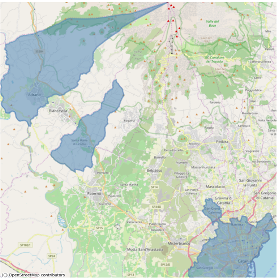
\includegraphics[width=.18\textwidth]{compgeo/map-biancavilla-in.png}};

\node[align=left, text width=.18\textwidth] (pixel-text-in) at (-.9*\width, 1*\height) {TARGET is between the towns of RED and LIME, 32 kilometres (20 mi) northwest of BLUE.};
\node (pixel-in) at (-.9*\width, -1*\height) {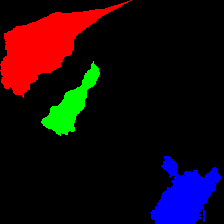
\includegraphics[width=.18\textwidth]{compgeo/pixel-biancavilla-in.png}};

\node[draw, fill=black!25, align=center, inner sep=5pt] (model) at (0*\width, 0*\height) {Multi-\\Modal\\Model};

\node (pixel-out) at (.9*\width, 0*\height) {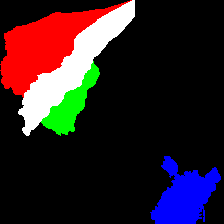
\includegraphics[width=.18\textwidth]{compgeo/pixel-biancavilla-out.png}};

\node (map-out) at (2*\width, 0*\height) {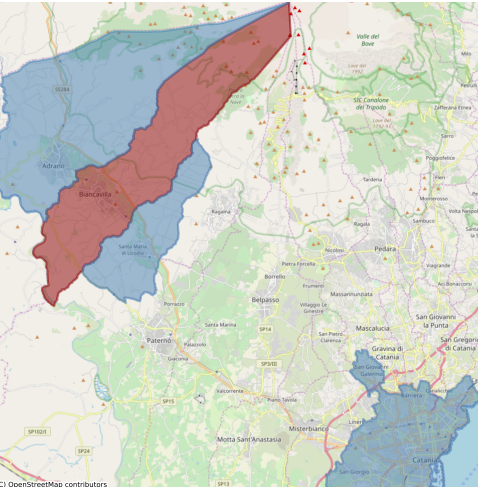
\includegraphics[width=.18\textwidth]{compgeo/map-biancavilla-out.png}};

\draw[-latex,thick] (text-in.east) -- (pixel-text-in.west);
\draw[-latex,thick] (map-in.east) -- (pixel-in.west);
\draw[-latex,thick] (pixel-text-in.east) -- (model);
\draw[-latex,thick] (pixel-in.east) -- (model);
\draw[-latex,thick] (model) -- (pixel-out);
\draw[-latex,thick] (pixel-out) -- (map-out);
\end{tikzpicture}
\end{frame}


\begin{frame}{Current language-vision models (LVMs) fall short}
\begin{columns}
\begin{column}{0.48\textwidth}
Input: \\
\smallskip
\begin{tabular}{ p{.65\textwidth} l @{}}
\textit{TARGET lies 6 km east of RED and south of the valley of the GREEN.} &
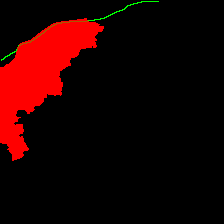
\includegraphics[align=t,width=.25\textwidth]{compgeo/GL006_046_oracle_input.png}
\end{tabular}

\medskip
Output: \\
\begin{tabular}{ l l l @{}}

\includegraphics[width=.25\textwidth]{compgeo/GL006_046_oracle_output_reference.png}
&

\includegraphics[width=.25\textwidth]{compgeo/GL006_046_oracle_output_clip.png}
&

\includegraphics[width=.25\textwidth]{compgeo/GL006_046_oracle_output_lisa.jpg}
\\
Expected & CLIP & LISA
\end{tabular}
\end{column}
\pause
\begin{column}{0.48\textwidth}
Input: \\
\smallskip
\begin{tabular}{ p{.65\textwidth} l @{}}
\textit{TARGET is ORANGE.} &
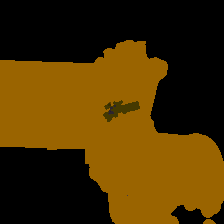
\includegraphics[align=t,width=.25\textwidth]{compgeo/GL024_425_color_input.png}
\end{tabular}

\medskip
Output: \\
\begin{tabular}{ l l l @{}}

\includegraphics[width=.25\textwidth]{compgeo/GL024_425_color_output_reference.png}
&

\includegraphics[width=.25\textwidth]{compgeo/GL024_425_color_output_clip.png}
&
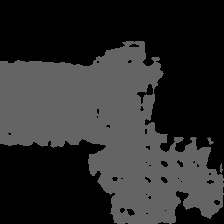
\includegraphics[width=.25\textwidth]{compgeo/GL024_425_color_output_lisa.jpg}
\\
Expected & CLIP & LISA
\end{tabular}
\end{column}
\end{columns}
\pause
\bigskip
\alert{Opportunity: can we train more multi-modal understanding into LVMs?}
\end{frame}

\section{Opportunity 2: Teaching LLMs to access external knowledge via code}

\begin{frame}[b]
\sectionbox
\hfill
\headshot{people/su-xin.jpg}{Xin Su}{Doctoral student}
\end{frame}

\subsection{Time expression normalization}

\begin{frame}{Time normalization as code generation}
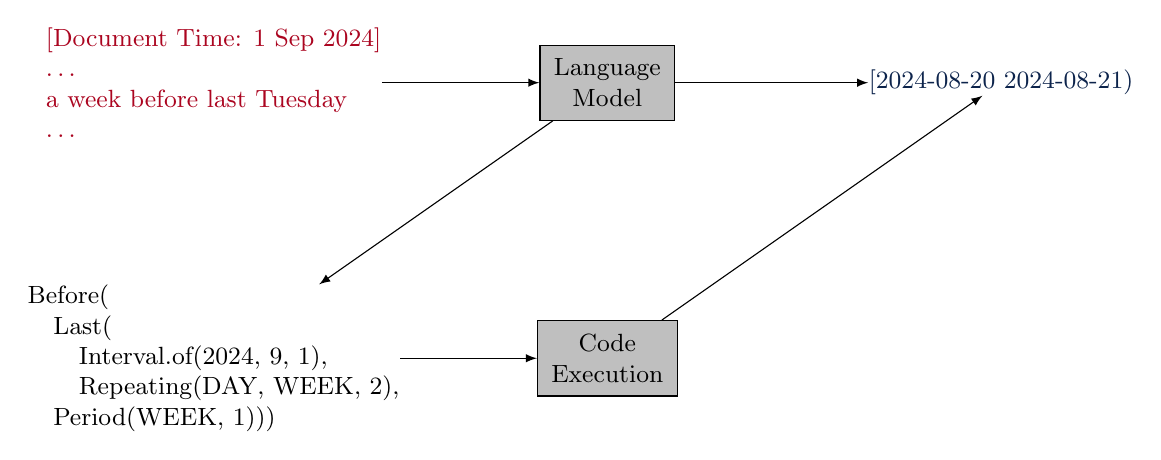
\begin{tikzpicture}[font=\small]
\pgfmathsetmacro{\height}{3.5}
\pgfmathsetmacro{\width}{5}

\node[text=ua-red, inner sep=0pt, align=left] (text) at (-1*\width, 0*\height) {[Document Time: 1 Sep 2024]\\\ldots\\a week before last Tuesday\\\ldots};

\node[draw, fill=black!25, align=center, inner sep=5pt] (model) at (0*\width, 0*\height) {Language \\ Model};

\node[text=ua-blue, inner sep=0pt, align=left] (iso) at (1*\width, 0*\height) {[2024-08-20 2024-08-21)};

\visible<2->{\node[align=left, inner sep=0pt] (code) at (-1*\width, -1*\height) {%
Before(\\
\quad Last(\\
\quad\quad Interval.of(2024, 9, 1), \\
\quad\quad Repeating(DAY, WEEK, 2), \\
\quad Period(WEEK, 1)))};}

\visible<2->{\node[draw, fill=black!25, align=center, inner sep=5pt] (execution) at (0*\width, -1*\height) {Code \\ Execution};}

\draw[-latex] (text) -- (model);
\invisible<2->{\draw[-latex] (model) -- (iso);}
\visible<2->{\draw[-latex] (model) -- (code);
\draw[-latex] (code) -- (execution);
\draw[-latex] (execution) -- (iso);}
\end{tikzpicture}
\end{frame}


\begin{frame}{Code generation + code execution \textgreater\ Direct generation}
Data:
\begin{itemize}
\item News articles from TempEval-2013 \parencite{uzzaman-etal-2013-semeval}
\item Compositional time annotations from \textcite{bethard-etal:2016:LREC}
\end{itemize}

\pause
\bigskip
\begin{tabular}{lc}
    \toprule
    \textbf{Model}  & \textbf{Accuracy} \\
    \midrule
    Claude 3.7 + direct prompted & 0.38 \\
    Claude 3.7 + code prompted + execution & 0.49 \\
    Qwen2.5-0.5B + code fine-tuned + execution & 0.01 \\
    \pause
    \quad + Claude-generated data & 0.59 \\
    \bottomrule
\end{tabular}

\pause
\bigskip
\alert{Opportunity: what other tasks could be formulated as code generation?}
\end{frame}


\begin{frame}
    \frametitle{Recap: Lessons and Opportunities}
    \tableofcontents
\end{frame}

\begin{frame}{Thanks!}
\begin{block}{Research leads}
\headshot{people/laparra-egoitz.jpg}{Egoitz Laparra, Ph.D.}{Postdoc}
\qquad
\headshot{people/xu-dongfang.jpeg}{Dongfang Xu, Ph.D.}{Doctoral student}
\qquad
\headshot{people/zhang-zeyu.png}{Zeyu Zhang, Ph.D.}{Doctoral student}
\qquad
\headshot{people/su-xin.jpg}{Xin Su}{Doctoral student}
\qquad
\headshot{people/wang-ruoyao.png}{Ruoyao Wang}{Doctoral student}
\end{block}
\begin{columns}
\begin{column}{0.65\textwidth}
\begin{block}{Grant collaborators}
\headshot{people/savova-guergana.jpg}{Guergana Savova, Ph.D.}{Boston Children's Hospital}
\headshot{people/surdeanu-mihai.jpeg}{Mihai Surdeanu, Ph.D.}{University of Arizona}
\headshot{people/lopez-hoffmann-laura.jpg}{Laura L\'{o}pez-Hoffman, Ph.D.}{University of Arizona}
\headshot{people/miller-timothy.jpg}{Timothy Miller, Ph.D.}{Boston Children's Hospital}
\end{block}
\end{column}
\hfill
\begin{column}{0.3\textwidth}
\begin{block}{Funding}
\scriptsize
\funding{funding/nih_nlm.png}{R01LM010090}

\funding{funding/darpa.png}{W911NF-18-1-0014}

\funding{funding/nih_nigms.jpg}{R01GM114355}

\funding{funding/nsf.png}{1831551}

\funding{funding/nih_nlm.png}{R01LM012918}
\end{block}
\end{column}
\end{columns}
\end{frame}


\appendix

\begin{frame}[allowframebreaks]{References}
\printbibliography
\end{frame}


\end{document}
